\documentclass[11pt,a4paper]{article}
\usepackage[margin=2.2cm]{geometry}
\usepackage{amsmath,amssymb}
\usepackage{graphicx}
\usepackage{booktabs}
\usepackage{xcolor}
\usepackage{float}
\usepackage{caption}
\usepackage{enumitem}
\usepackage[colorlinks=true,linkcolor=blue!50!black,urlcolor=blue!50!black,citecolor=blue!50!black]{hyperref}
\graphicspath{{../results/figures/}}
\setlist{itemsep=2pt,topsep=4pt}
\setlength{\emergencystretch}{3em}
\usepackage{microtype}
\newcommand{\IBM}{\textsc{ibm}}
\newcommand{\pstar}{p^{*}}
\title{\textbf{Antagonistic alleles: deterministic theory versus\\ zero-leakage individual-based emulation}\\[4pt]
\large Expert report}
\author{Reconstruction and verification of Samant, Moitra, Sinha \& Prasad (IISER Mohali poster),\\
Parsons (1961), Owen (1953), Havird \emph{et al.}\ (2019) and classical sexual-antagonism theory}
\date{5 October 2026}

\begin{document}
\maketitle

\begin{abstract}
Every model was implemented twice. The first implementation is a deterministic \emph{oracle}: the papers' recursions, solved exactly. The second is a stochastic individual-based model (\IBM) built only from biological primitives: sex assignment, Bernoulli viability, uniform choice of surviving parents, and Mendelian or maternal transmission with crossover. The \IBM\ never evaluates a recursion, equilibrium or eigenvalue, and a test enforces this. Both engines receive identical \emph{conditions} (viability tables, $r$, $N$, founding genotypes).

The reconstructed poster model reproduces the poster's $\pstar$ exactly and its invasion thresholds to $\le 0.002$ in $a$. The \IBM\ agrees with the oracle's direction of modifier spread in 99\% of decided cells. Parsons' invasion conditions hold in 100\% of decided cells. Kidwell/Fry/Rice protected-polymorphism conditions hold in 98--100\%.

Where the \IBM\ departs from the oracle, the departure is a finite-population effect that a stochastic theory predicts:
\begin{itemize}
\item drift-induced loss of the IaSC polymorphism (diffusion times, error 3.7\% median after an $N_e$ calibration);
\item failure of Kimura's sex-averaged fixation probability under strong antagonism (corrected by the full diffusion);
\item probabilistic, $N$-sharpening bistability thresholds.
\end{itemize}
An analysis-only ML layer (a Gaussian-process boundary denoiser, a neural emulator and simulation-based inference) recovers the theoretical structure from \IBM\ data alone.
\end{abstract}

\tableofcontents
\newpage

%=====================================================================
\section{Sources and scope}
\begin{tabular}{p{4.6cm}p{5.2cm}p{5.6cm}}
\toprule
Document & Content & Treatment\\
\midrule
Poster (Samant \emph{et al.}) & Two-locus haploid IaSC + modifier; linear stability, bifurcations, basins & Full reconstruction; \IBM\ counterpart for each panel\\
Parsons (1961) & Latent-root invasion conditions (autosomal, X-linked) & Oracle + \IBM; Owen (1953) bistability\\
Havird \emph{et al.}\ (2019) & Review: mother's curse, twofold rule, restorers & Formalised cytonuclear model + \IBM\\
Morrow \emph{et al.}\ (2003) & Experimental harm in insects (ANOVA) & Context only (no model)\\
AI blueprint (.txt) & Owen/Mandel cubic, zero-leakage design & Cubic verified (4{,}000/4{,}000 random sets)\\
Kidwell 1977; Rice 1984/87; Fry 2010; Kimura 1962 & Classical SA and diffusion results & Extended test suite (\S\ref{sec:ext})\\
\bottomrule
\end{tabular}

%=====================================================================
\section{Architecture and the zero-leakage contract}
\begin{itemize}
\item \texttt{config.py} is the single source of conditions and seeds. Seeds are derived from \texttt{MASTER\_SEED} and the experiment name, so each experiment reproduces independently.
\item \texttt{deterministic/} holds the oracles: the poster map with a sympy Jacobian; Owen/Parsons; the mother's-curse model; and the classical SA results with Kimura and backward-Kolmogorov solvers.
\item \texttt{ibm/} holds the simulators: numba kernels (haploid two-locus, diploid with maternal cytoplasm, X-linked, and XY with genetic sex determination) and optional OpenCL kernels for AMD GPUs.
\item The \IBM\ never imports \texttt{deterministic/}, sympy or scipy (enforced by a test).
\item Frequencies are only counted for the record. Even the poster's IaSC starting state is reached by an \IBM\ burn-in rather than set to $\pstar$.
\end{itemize}

\noindent\textbf{One \IBM\ generation:}
\begin{enumerate}
\item Assign sex (a fair coin, or the inherited Y in the XY kernel).
\item Each individual survives with probability $w_{\text{sex},g}/\max_g w_{\text{sex},g}$.
\item Each of $N$ offspring picks a uniformly random surviving mother and father.
\item Gametes form by segregation, with a crossover with probability $r$. The cytoplasm is maternal.
\end{enumerate}
GPU kernels draw parents by rejection sampling among survivors, which is exactly uniform. They use counter-based (splitmix64) random numbers and were validated against the CPU kernels by KS tests on 400 replicate populations.

%=====================================================================
\section{The poster model}
\subsection{Reconstruction}
Haplotypes $x=(x_{11},x_{12},x_{21},x_{22})=(A_1M_1,A_1M_2,A_2M_1,A_2M_2)$.

\begin{center}\begin{tabular}{lcccc}\toprule
 & $A_1M_1$ & $A_1M_2$ & $A_2M_1$ & $A_2M_2$\\\midrule
males & $1+a$ & $1+a$ & $1$ & $1$\\
females & $1+bk_1$ & $1$ & $1+bk_2$ & $1+b$\\\bottomrule\end{tabular}\end{center}

\noindent\textbf{Life cycle} (not stated on the poster; this is the one that reproduces its formulas):
\begin{enumerate}
\item haploid selection in each sex, $m_{ij}=x_{ij}w^m_{ij}/\bar w_m$ and $f_{ij}=x_{ij}w^f_{ij}/\bar w_f$;
\item random union of one female and one male haplotype;
\item meiosis with recombination $r$:
\begin{equation}
x'_{ij}=\tfrac12(1-r)(f_{ij}+m_{ij})+\tfrac12 r\,(f_{A_i}m_{M_j}+m_{A_i}f_{M_j}).
\end{equation}
\end{enumerate}

\noindent\textbf{One locus.} The recursion is $p'=\tfrac12\big[p(1+a)/(1+ap)+p/(1+b(1-p))\big]$. Its fixed points satisfy
\[
p\,[2ab\,p^2-(a-b+3ab)p+(a-b+ab)]=0,
\]
with roots $p=0$, $p=1$ and
\begin{equation}\pstar=\frac{ab+a-b}{2ab}=\tfrac12+\tfrac12\Big(\frac1b-\frac1a\Big),\end{equation}
exactly as on the poster. The root is interior iff $-1<1/b-1/a<1$, i.e.\ $a\in(b/(1+b),\,b/(1-b))$, which is $(1/6,1/4)$ for $b=0.2$. The restoring eigenvalue $\mu=dp'/dp|_{\pstar}\in[0.9917,\,0.99997]$: the polymorphism is stable, but only weakly.

\subsection{Invasion of the modifier: closed form}
The face $x_{11}=x_{21}=0$ is invariant, so the Jacobian at $(0,\pstar,0)$ is block-triangular. Its eigenvalues are $\mu$ and those of a $2\times2$ matrix $B$, and \textbf{M$_1$ invades $\iff\rho(B)>1$}.

The Jacobian was derived with sympy and checked against finite differences ($<10^{-10}$). A hand-derived closed form agrees with sympy to $10^{-12}$. Let
\[
W_m=1+a\pstar,\quad W_f=1+b(1-\pstar),\quad \varphi_m=\frac{\pstar(1+a)}{W_m},\quad \varphi_f=\frac{\pstar}{W_f},
\]
\[
\alpha=\frac{1+a}{W_m},\quad \gamma=\frac{1}{W_m},\quad \beta_i=\frac{1+bk_i}{W_f}.
\]
Then
\begin{align}
B_{11}&=\tfrac12(1-r)(\beta_1+\alpha)+\tfrac12 r(\varphi_f\alpha+\varphi_m\beta_1), &
B_{12}&=\tfrac12 r(\varphi_f\gamma+\varphi_m\beta_2),\\
B_{21}&=\tfrac12 r((1-\varphi_f)\alpha+(1-\varphi_m)\beta_1), &
B_{22}&=\tfrac12(1-r)(\beta_2+\gamma)+\tfrac12 r((1-\varphi_f)\gamma+(1-\varphi_m)\beta_2).
\end{align}
At $r\to0$ the eigenvalues are $1+bk_1/(2W_f)$ and $1-b(1-k_2)/(2W_f)$. So \emph{any} $k_1>0$ invades on the $A_1$ background, which is the thin unstable strip along $r\approx0$ in the poster's panels. Recombination moves M$_1$ onto $A_2$, where it costs $b(1-k_2)$. This is the analytic reason that low $r$ favours resolution (poster result 4). A larger $a$ raises $\pstar$, putting more M$_1$ on $A_1$ (poster result 3).

\subsection{Reproduction of the poster}
\begin{table}[H]\centering
\caption{Invasion thresholds along $a$ at $r=0.1$, $b=0.2$ (bifurcation diagram, starting near the fixed point).}
\begin{tabular}{lccc}\toprule
$(k_1,k_2)$ & reconstruction & poster (read) & stable fraction, $b=0.2$ / $0.02$\\\midrule
(0.2, 0.2) & 0.2142 & $\approx$0.212 & 0.612 / 0.781\\
(0.8, 0.8) & 0.1710 & $\approx$0.169 & 0.089 / 0.178\\
(0.5, 0.5) & 0.1855 & $\approx$0.184 & 0.288 / 0.467\\
(0.2, 0.8) & 0.1940 & $\approx$0.193 & 0.340 / 0.479\\
(0.8, 0.2) & 0.1780 & $\approx$0.176 & 0.248 / 0.456\\
(0.5, 1.0) & 0.1668 & $\approx$0.166 & 0.000 / 0.000\\
(0.0, 0.5) & never & never & 1.000 / 1.000\\\bottomrule
\end{tabular}\end{table}
All five summary results on the poster are reproduced: $k_2<1$ does not guarantee resolution; stronger selection widens resolution; larger $a$ helps; lower $r$ helps; and small-effect modifiers are hypersensitive.

\begin{figure}[H]\centering
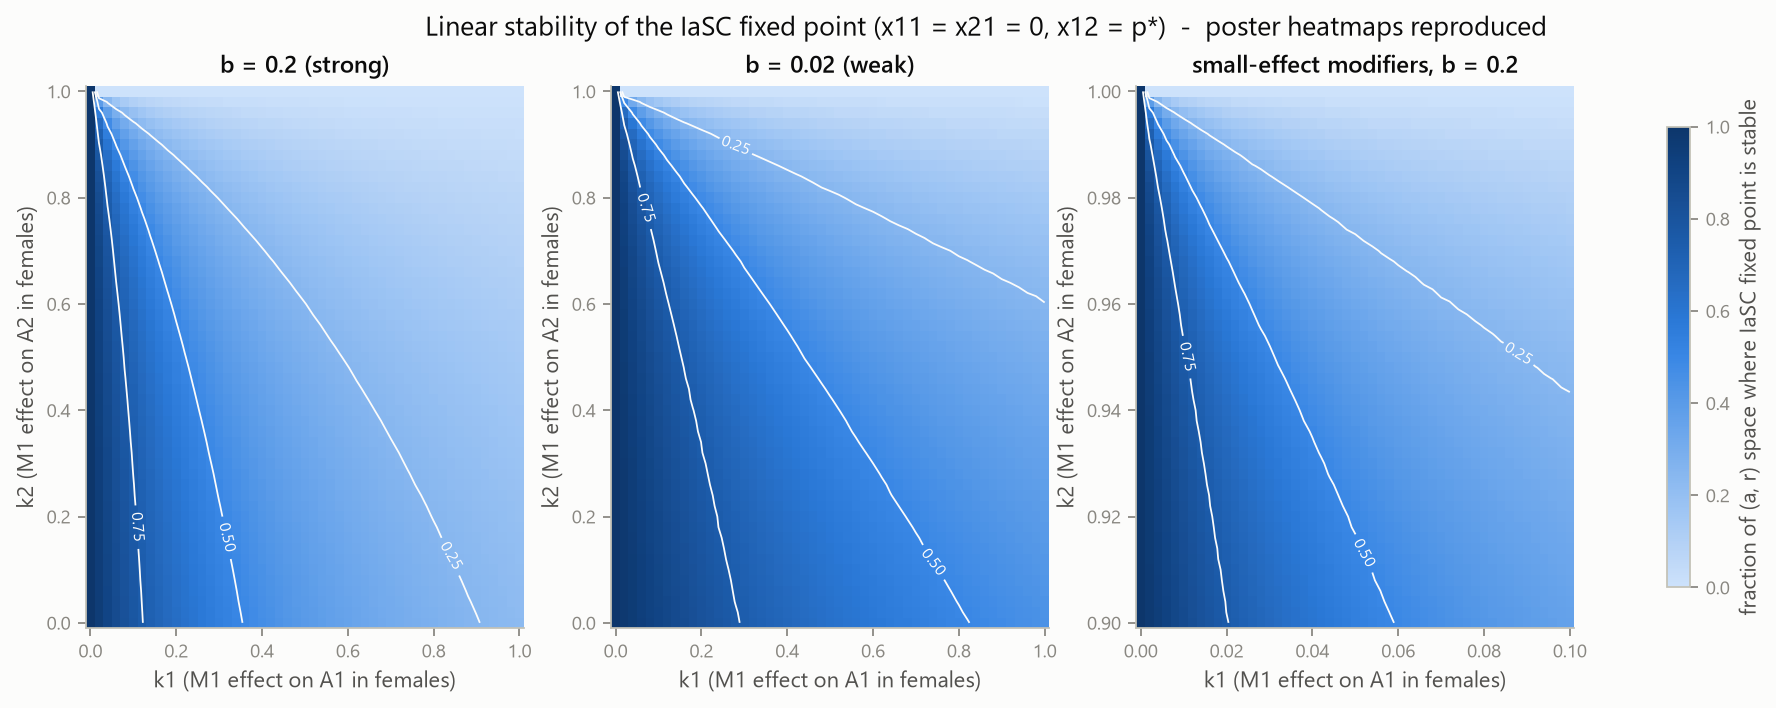
\includegraphics[width=\textwidth]{P1_stability_heatmaps.png}
\caption{Fraction of the $(a,r)$ rectangle in which the IaSC point is stable. Reproduces the poster heatmaps.}\end{figure}
\begin{figure}[H]\centering
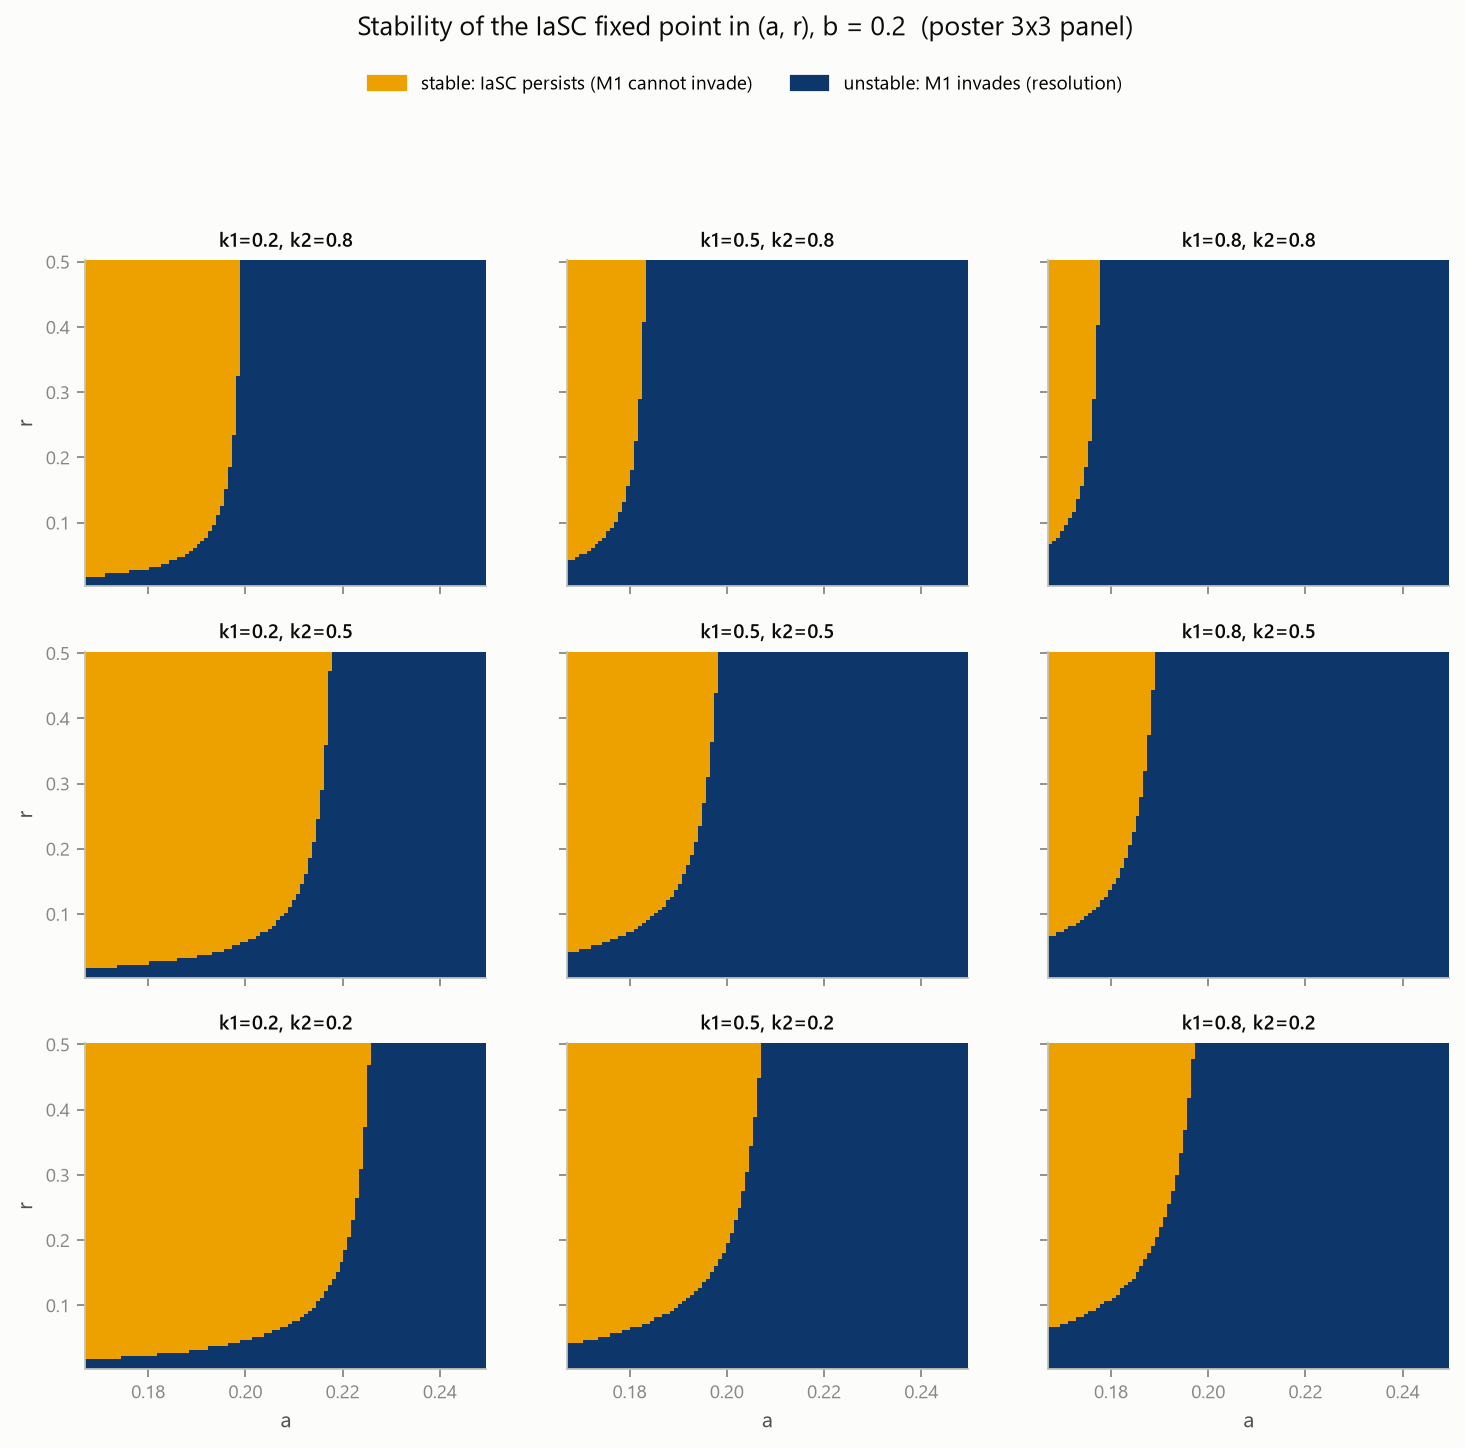
\includegraphics[width=0.78\textwidth]{P2a_ar_stability_grid.png}
\caption{Stable (IaSC persists) and unstable (M$_1$ invades) zones in $(a,r)$ for $k_1,k_2\in\{0.2,0.5,0.8\}$.}\end{figure}

\subsection{Confrontation with the IBM}
\begin{itemize}
\item \textbf{Polymorphism (P0).} The \IBM\ time-average tracks $\pstar$: RMSE $0.125$ at $N=500$ and $0.016$ at $N=5000$.
\item \textbf{Invasion (P2).} In 105 cells, each \IBM\ population first reaches its own IaSC state by burn-in. Then 2\% of individuals mutate to M$_1$, and we test the ensemble-mean change over 300 generations (95\% CI).
  \begin{itemize}
  \item Verdicts: 71 spread, 27 decline, 7 unresolved.
  \item The direction agrees with the oracle trajectory from the same dose in \textbf{99.0\%} of decided cells, and with the linear-stability sign in 94.9\%.
  \item $\mathrm{corr}(\log)=0.935$ between \IBM\ and oracle spread.
  \item The single disagreement is at $\lambda=0.9978$, close to neutral.
  \end{itemize}
\item \textbf{Thresholds (P4).} The bistability threshold becomes a sigmoid in the \IBM. Its midpoint approaches the oracle threshold and its width shrinks with $N$ (Table~\ref{tab:thr}).
\item \textbf{Basins and fates (P5, P7).} Per-initial-condition basin agreement is 0.88 for $(0.2,0.2)$ and 0.68 for $(0,0.5)$, where M$_1$ is neutral on $A_1$. Fate agreement in the animation is 84\%.
\item \textbf{Convergence (P6).} The between-population SD scales as $N^{-0.61}$ (95\% CI $-0.81$ to $-0.40$) for $N\ge1000$, consistent with $N^{-1/2}$. It is steeper ($-0.76$) when small $N$ is included, because stochastic loss of M$_1$ adds a second source of variance.
\end{itemize}
\begin{table}[H]\centering\caption{Bistability threshold: logistic fits to \IBM\ $P(\text{resolution})$ vs initial M$_1$ dose, $(k_1,k_2)=(0.2,0.2)$, $r=0.1$.}\label{tab:thr}
\begin{tabular}{lcccc}\toprule
$a$ & oracle threshold & $N=500$ & $N=2000$ & $N=6000$\\\midrule
0.190 & 0.415 & 0.569 (w 0.160) & 0.425 (w 0.085) & 0.387 (w 0.044)\\
0.205 & 0.109 & 0.211 (w 0.104) & 0.132 (w 0.056) & 0.116 (w 0.035)\\\bottomrule\end{tabular}\end{table}

\begin{figure}[H]\centering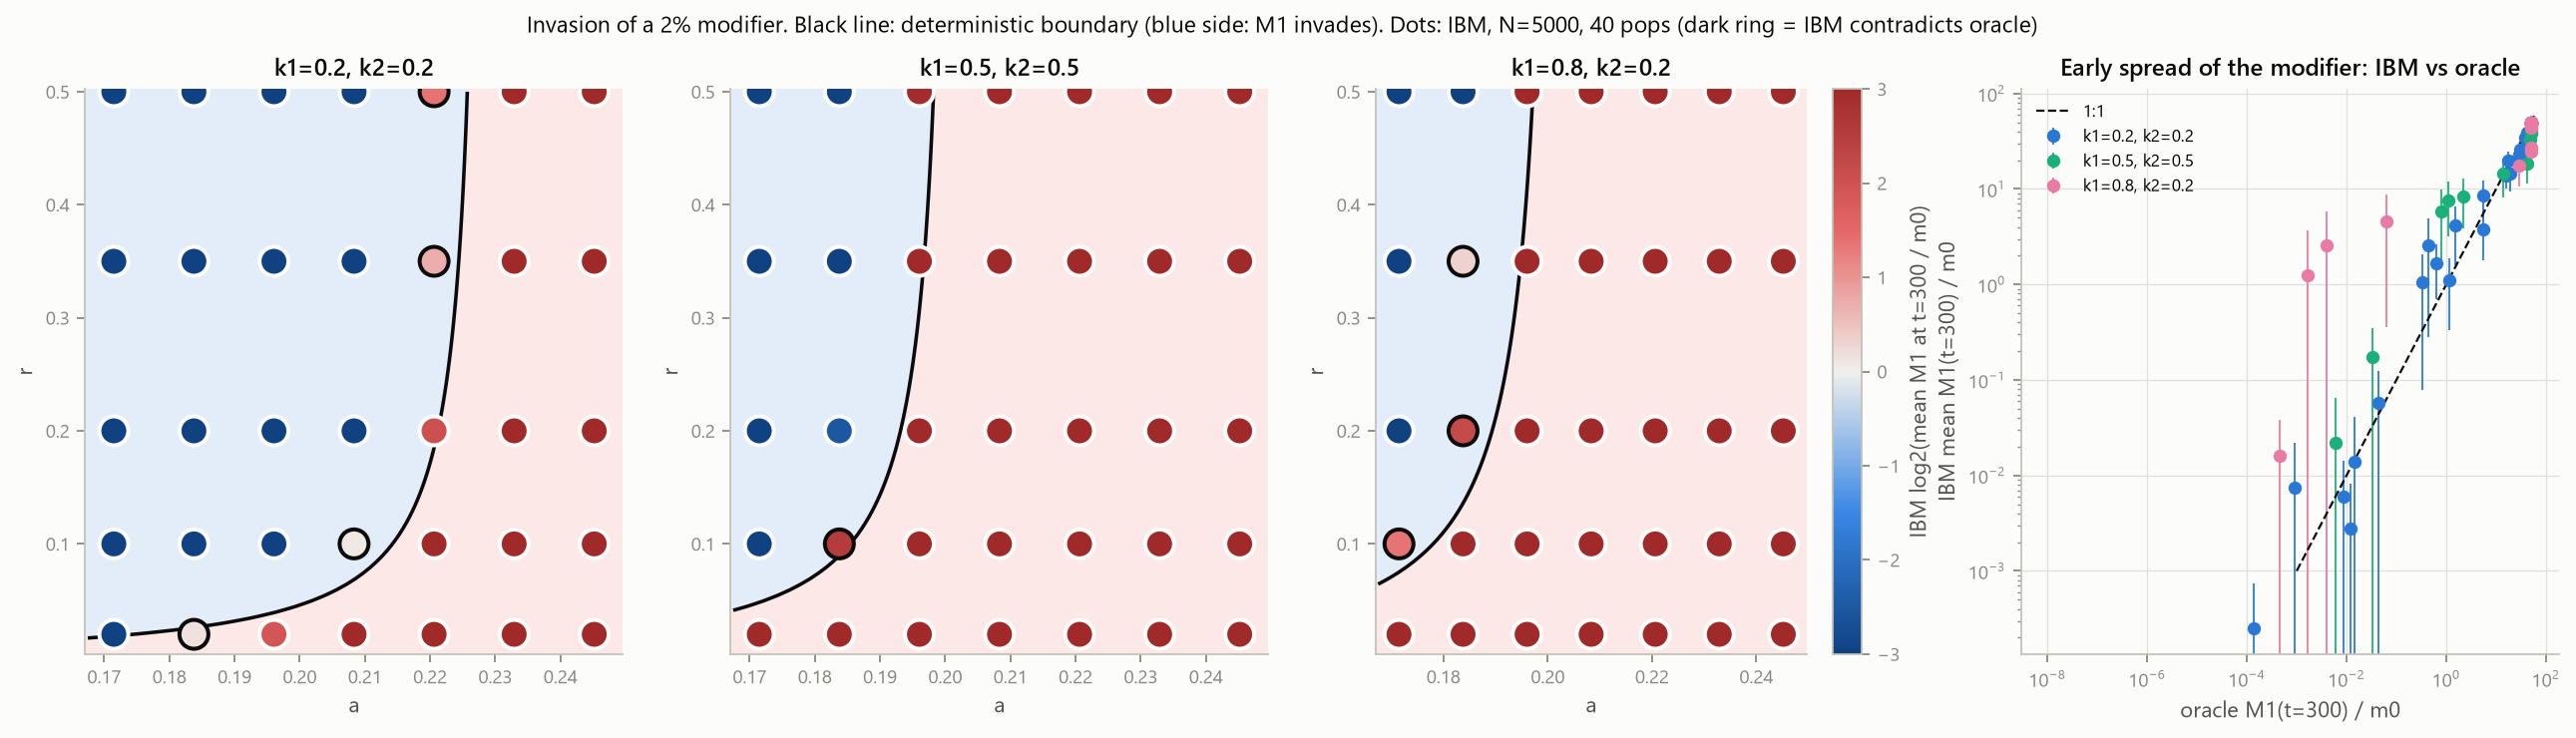
\includegraphics[width=\textwidth]{P2b_invasion_ibm_vs_boundary.png}
\caption{Deterministic invasion boundary vs \IBM\ early spread (log$_2$ ratio). Right: IBM vs oracle on a 1:1 plot.}\end{figure}
\begin{figure}[H]\centering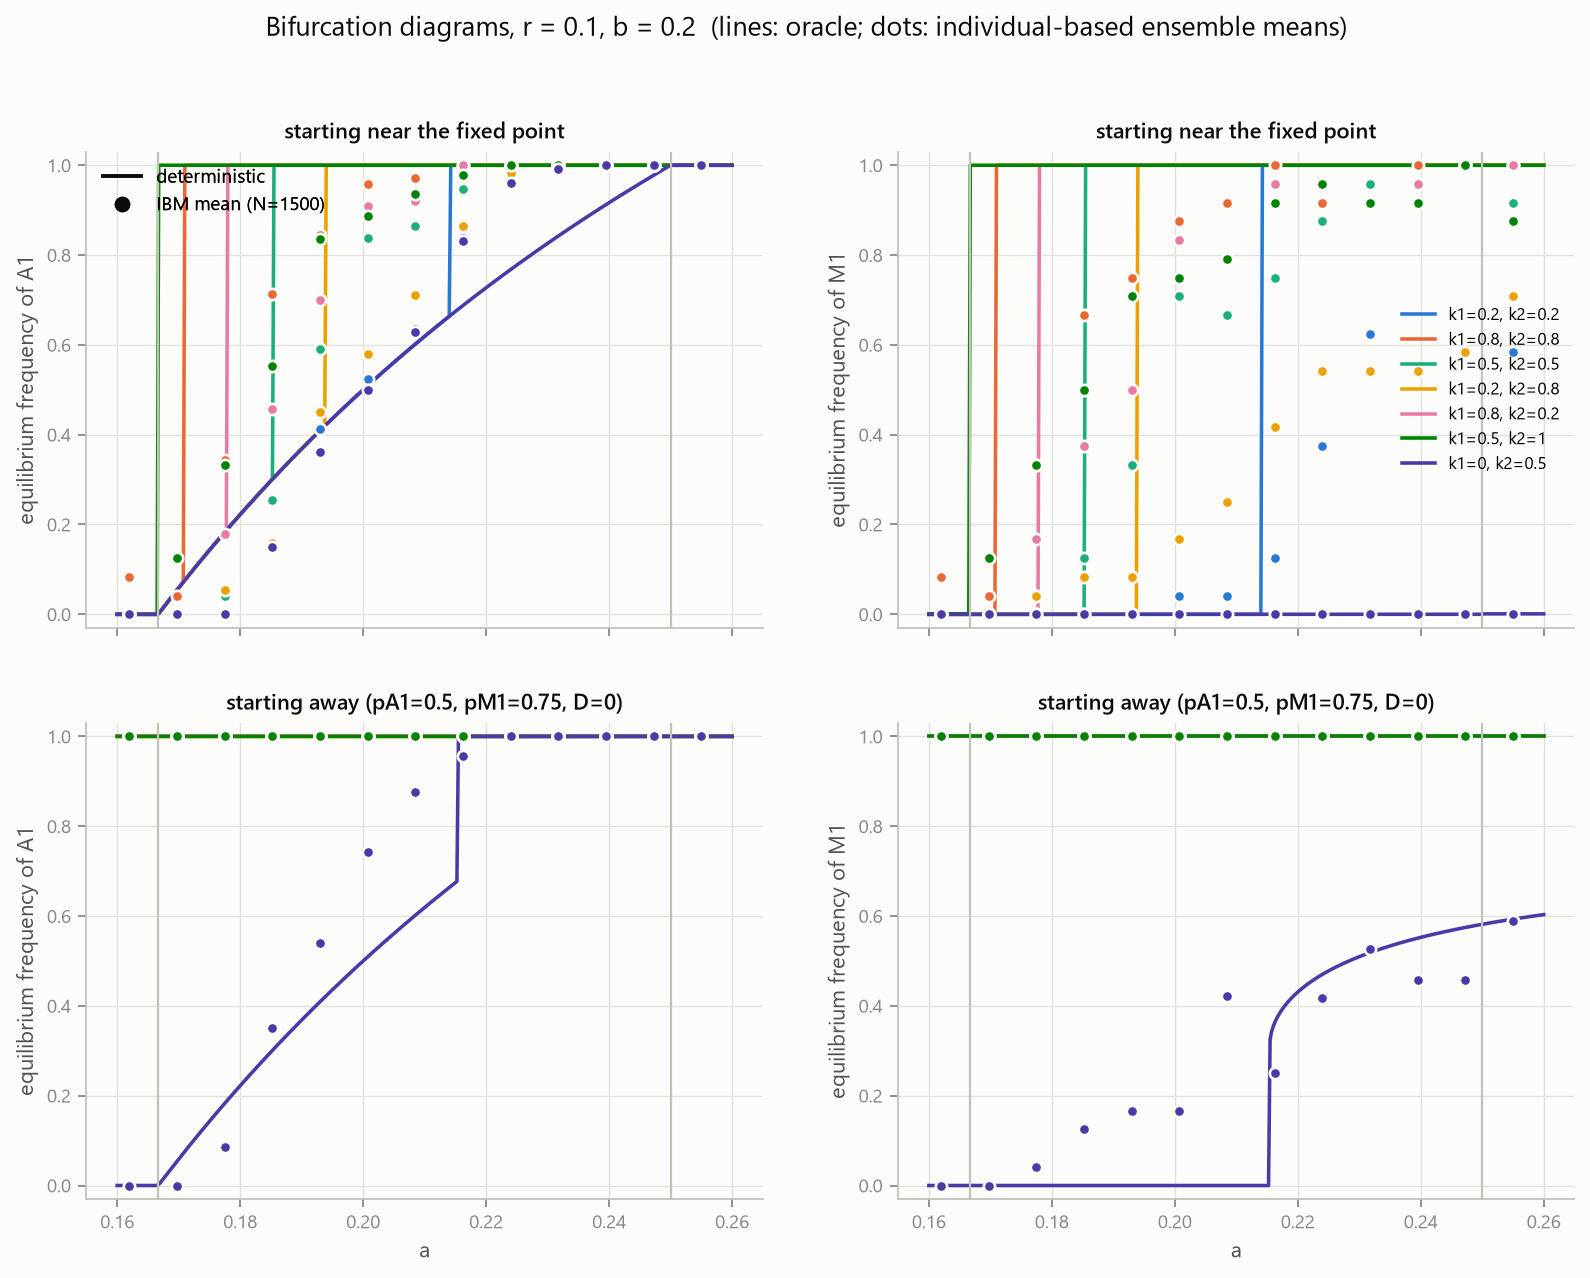
\includegraphics[width=0.9\textwidth]{P3_bifurcation.png}
\caption{Bifurcation diagrams (lines: oracle; dots: \IBM\ ensemble means). In the \IBM\ the oracle's jumps become ramps, because a finite dose establishes only with a probability.}\end{figure}
\begin{figure}[H]\centering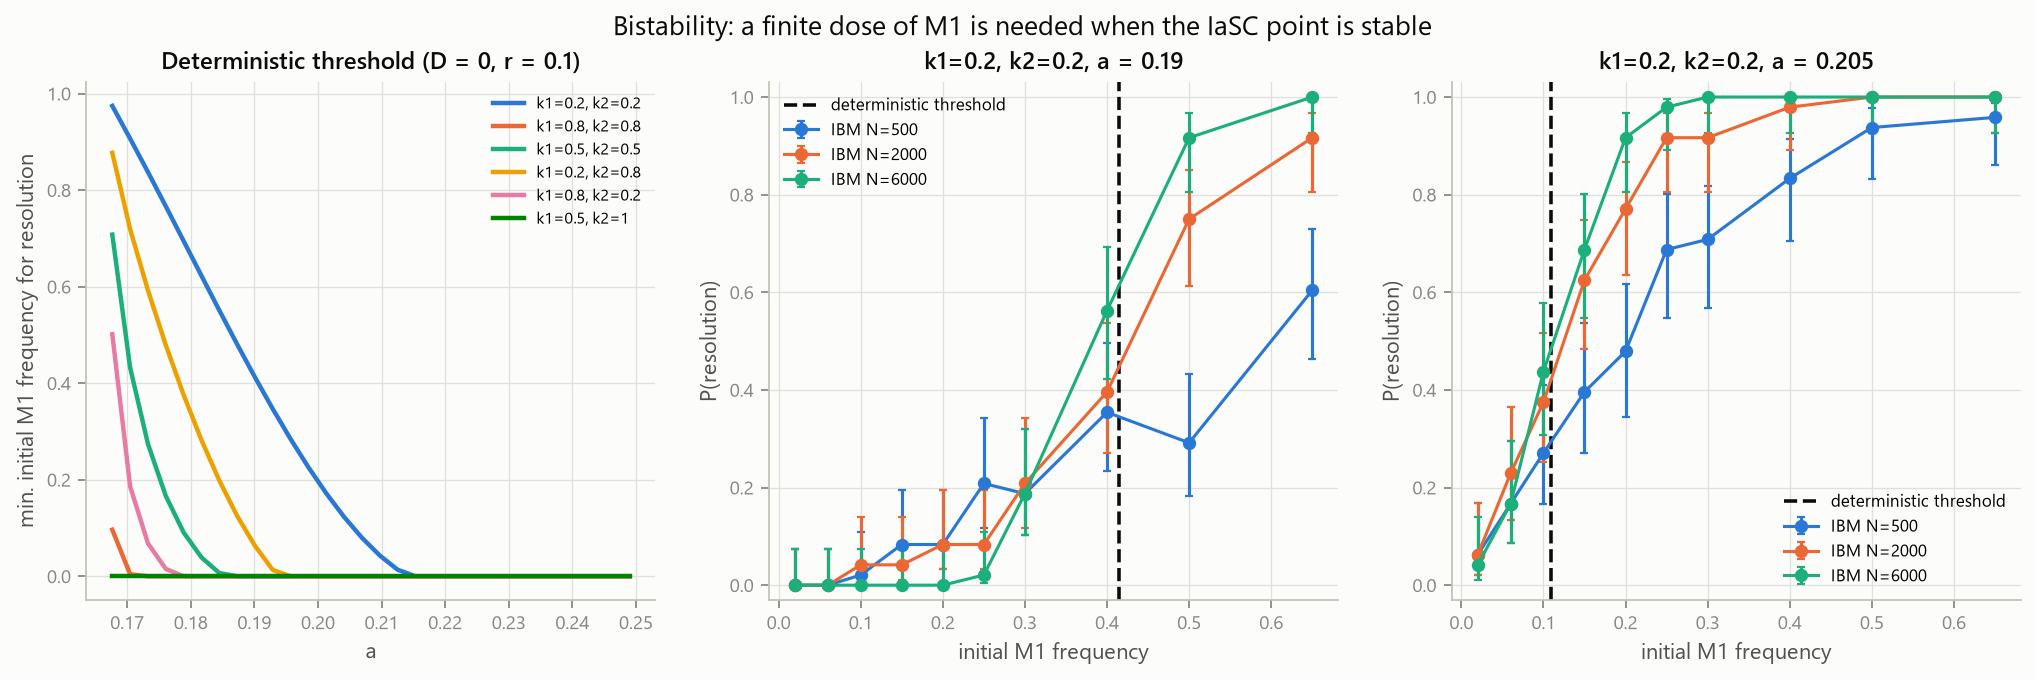
\includegraphics[width=\textwidth]{P4_thresholds.png}\caption{Thresholds: oracle (left) and \IBM\ sigmoids that sharpen with $N$.}\end{figure}
\begin{figure}[H]\centering
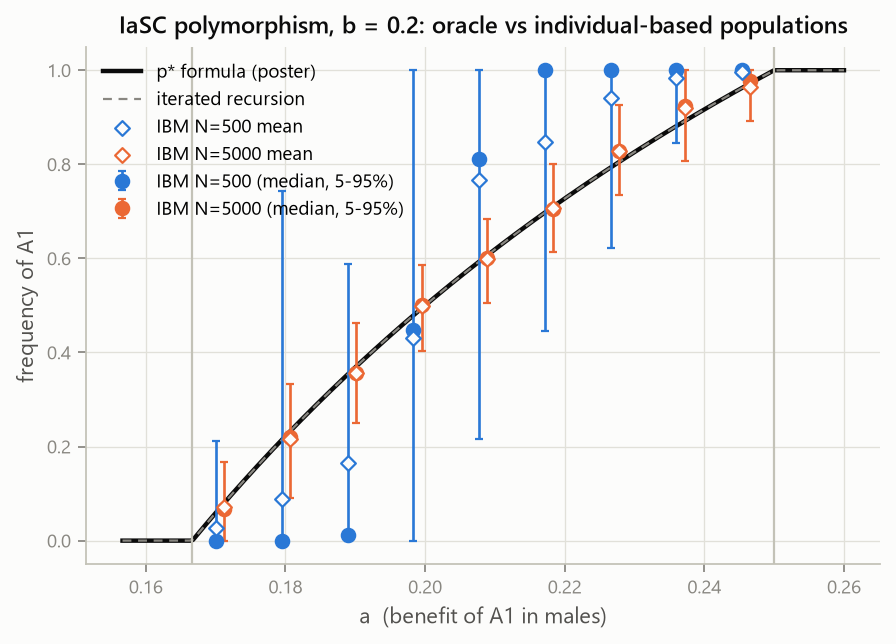
\includegraphics[width=0.49\textwidth]{P0_one_locus.png}\hfill
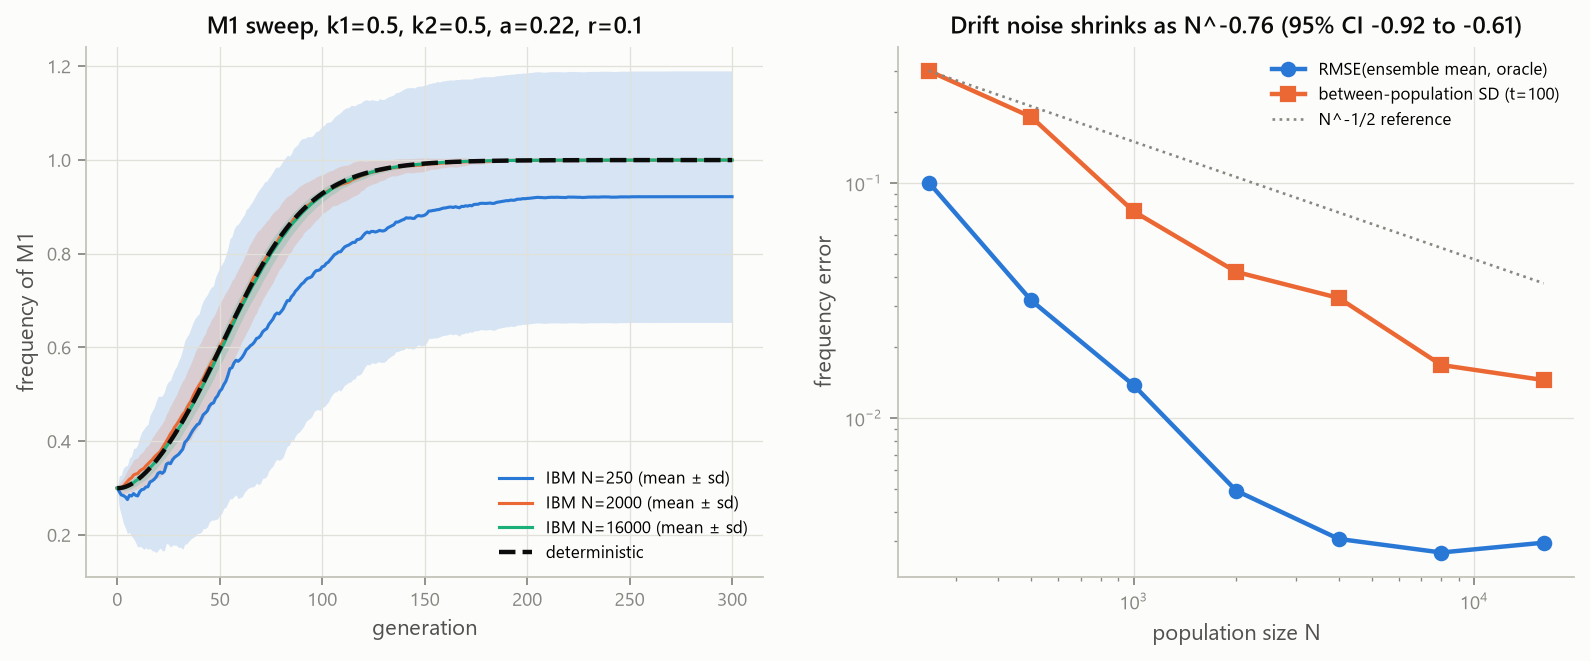
\includegraphics[width=0.49\textwidth]{P6_convergence.png}
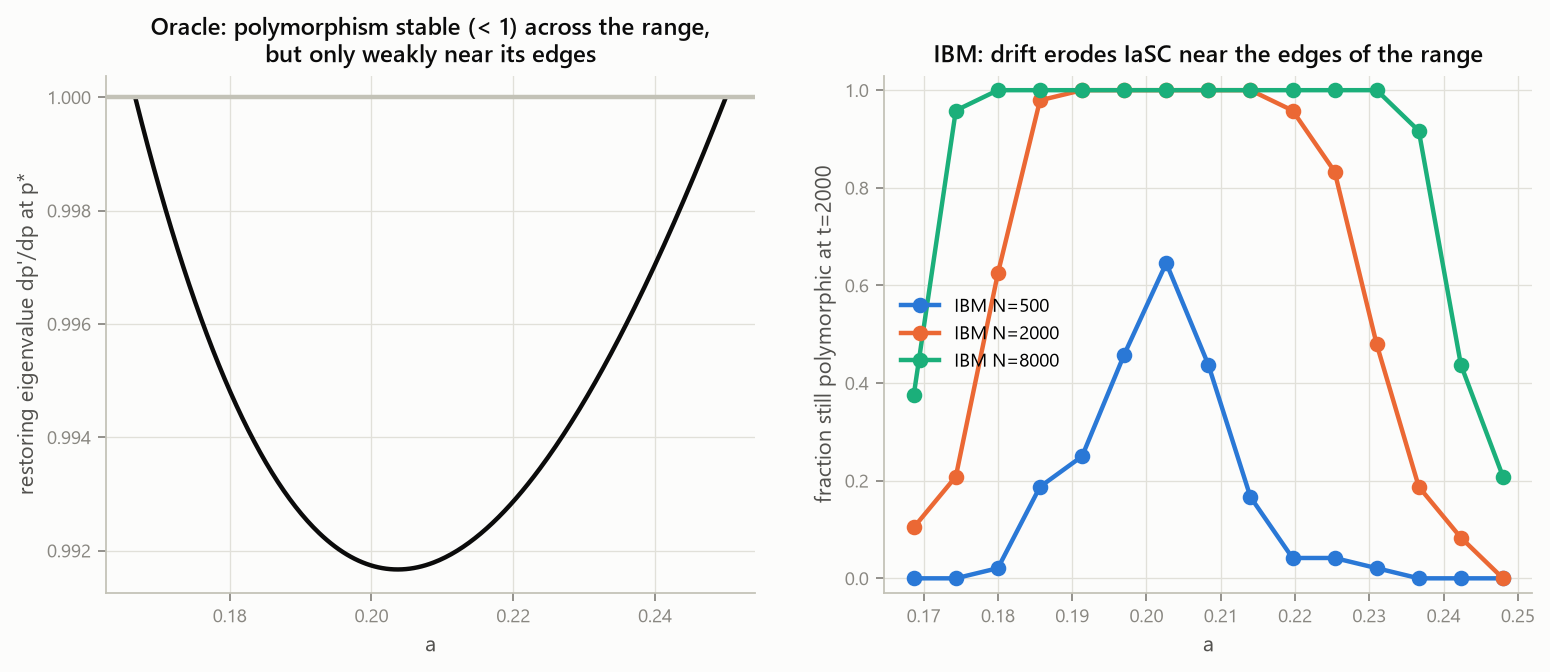
\includegraphics[width=0.9\textwidth]{P2c_persistence.png}
\caption{IaSC polymorphism vs $\pstar$; convergence with $N$; drift erodes IaSC near the edges of the $a$-range.}\end{figure}

\subsection{Unresolved points}
\begin{itemize}
\item The ``away from the fixed point'' panel does not state its initial condition. We used $(p_{A_1},p_{M_1},D)=(0.5,0.75,0)$. The orange plateau ($M_1=0.75$ for $a<1/6$) is not an attractor of the reconstructed map.
\item Also open: the domain behind ``fraction of parameter space'' (we used $a\in(b/(1+b),b/(1-b))$, $r\in(0,0.5]$), and the $r$ used in the size-of-perturbation panel (we assumed 0.1).
\end{itemize}

%=====================================================================
\section{Parsons (1961) and Owen (1953)}
\textbf{Autosomal.} Females have viabilities $(a_1,h_1,b_1)$ and males $(a_2,h_2,b_2)$ for $AA,Aa,aa$:
\[
p_i'=\frac{a_ip_1p_2+\tfrac12h_i(p_1q_2+p_2q_1)}{a_ip_1p_2+h_i(p_1q_2+p_2q_1)+b_iq_1q_2}.
\]
At $p=0$, $\lambda=\tfrac12(h_1/b_1+h_2/b_2)$, so A invades iff $h_1b_2+h_2b_1>2b_1b_2$ (eq.\ 2.5).

\textbf{X-linked.} Males follow $p_2'=a_2p_1/(a_2p_1+b_2q_1)$, and $\lambda^2-\tfrac{h_1}{2b_1}\lambda-\tfrac{h_1a_2}{2b_1b_2}=0$, so A invades iff $h_1(a_2+b_2)>2b_1b_2$, which is $\approx 2\beta_1+\beta_2-\alpha_2>0$ (eq.\ 3.6). The factor 2 is missing from the scanned ``note added in proof''; we read that as a scan artefact.

\textbf{Results.}
\begin{itemize}
\item Invasion verdicts agree with the oracle in \textbf{100\%} of decided cells, both autosomal and X-linked.
\item The worked example ($\beta_1=0.05$, $\beta_2=-0.02$, $\lambda=1.0165$) reaches the oracle equilibrium 0.4399; the \IBM\ median is 0.4402.
\item With Owen's two stable interior equilibria, \IBM\ basin agreement is \textbf{100\%}.
\item The blueprint's Mandel cubic matches our numeric equilibrium solver in 4{,}000/4{,}000 random parameter sets.
\end{itemize}
\begin{figure}[H]\centering
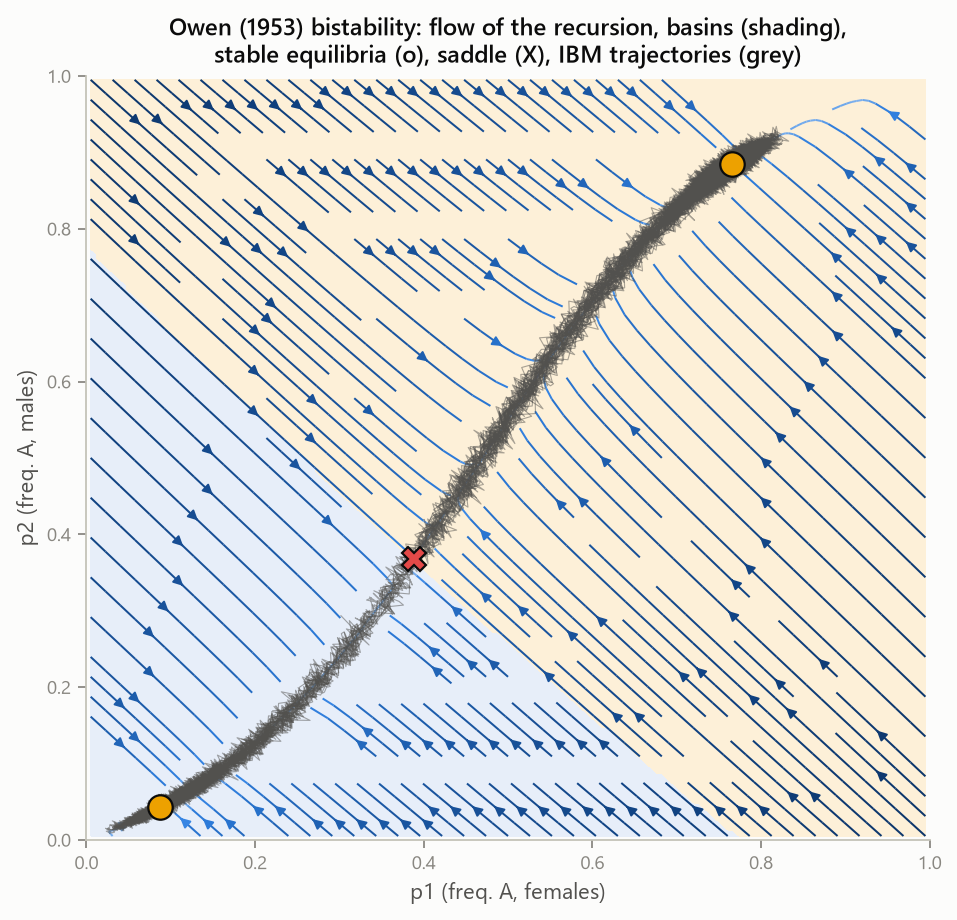
\includegraphics[width=0.53\textwidth]{O4_owen_phase_portrait.png}\hfill
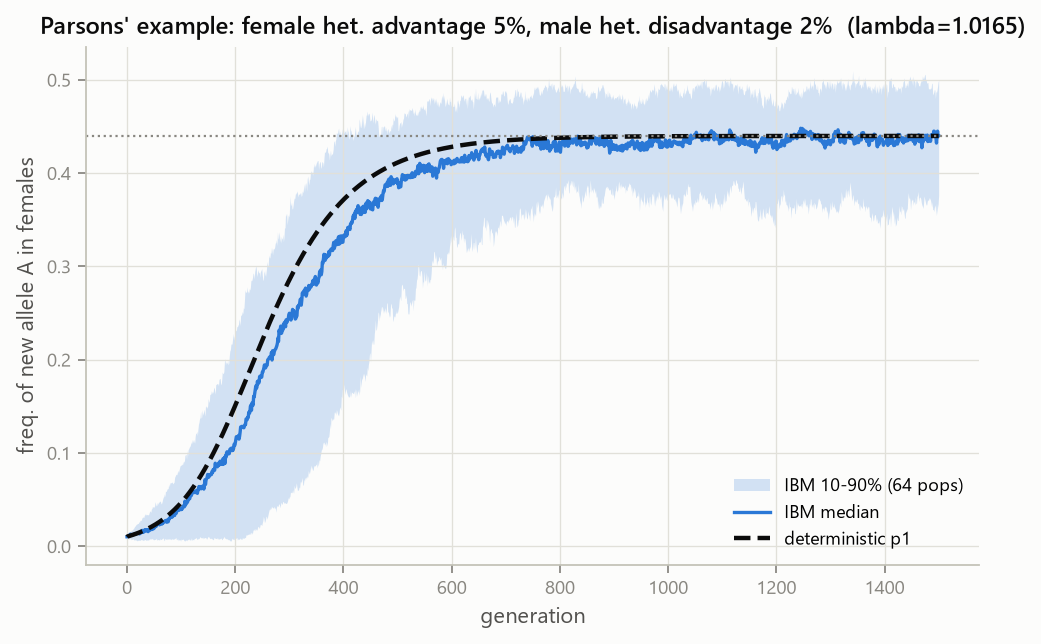
\includegraphics[width=0.45\textwidth]{O2_parsons_example.png}
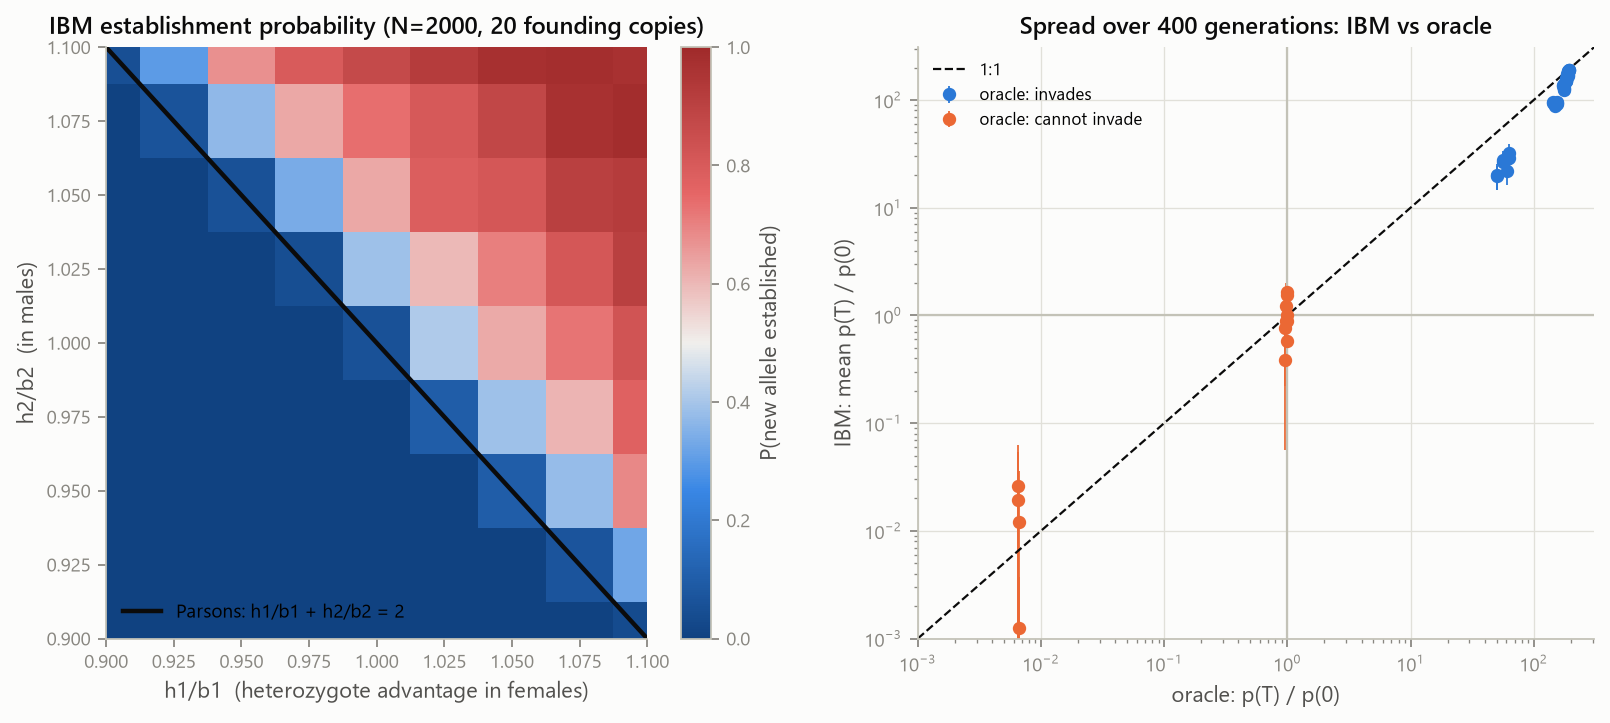
\includegraphics[width=\textwidth]{O1_autosomal_invasion.png}
\caption{Owen bistability (streamplot, basins, \IBM\ trajectories); Parsons' example; establishment map and IBM-vs-oracle spread.}\end{figure}

%=====================================================================
\section{Mother's curse (Havird \emph{et al.}\ 2019), formalised}
\textbf{Model.} The state is the zygote distribution $Z[c,g]$: mito type $c$ (maternal) and copies $g$ of a nuclear restorer. Viabilities are
\[
\text{females: }(1+s_fc)(1-\kappa\,d_g),\qquad \text{males: }(1-s_mc(1-\rho\,d_g))(1-\kappa\,d_g).
\]

\textbf{Predictions.}
\begin{itemize}
\item A rare mito variant grows by $1+s_f$, independent of $s_m$.
\item For a nuclear analogue, Parsons' root gives $\lambda=\tfrac12(w_{f,\text{het}}+w_{m,\text{het}})$. With sterile males ($w_m=0$) this requires $w_f>2$: the review's ``twofold'' statement is a special case of Parsons' eq.\ 2.5.
\end{itemize}

\textbf{Results.}
\begin{itemize}
\item Endpoint distributions do not depend on $s_m$ (KS $p=0.90,0.56,0.80$).
\item Twofold rule: 94\% agreement. The one exception, a nuclear allele with female fitness 2.1 ($\lambda=1.05$), invades only to an equilibrium of 4.5\%, which drift often erases.
\item Weak form: $P_{\text{fix}}=0.090, 0.108, 0.100$ for $s_m=0,0.5,1$ (neutral expectation 0.1).
\item The restorer fixes in 94\% of populations when it arises together with the mito variant, in 100\% when it arises after the sweep, and in 0\% without the variant.
\end{itemize}
\begin{figure}[H]\centering
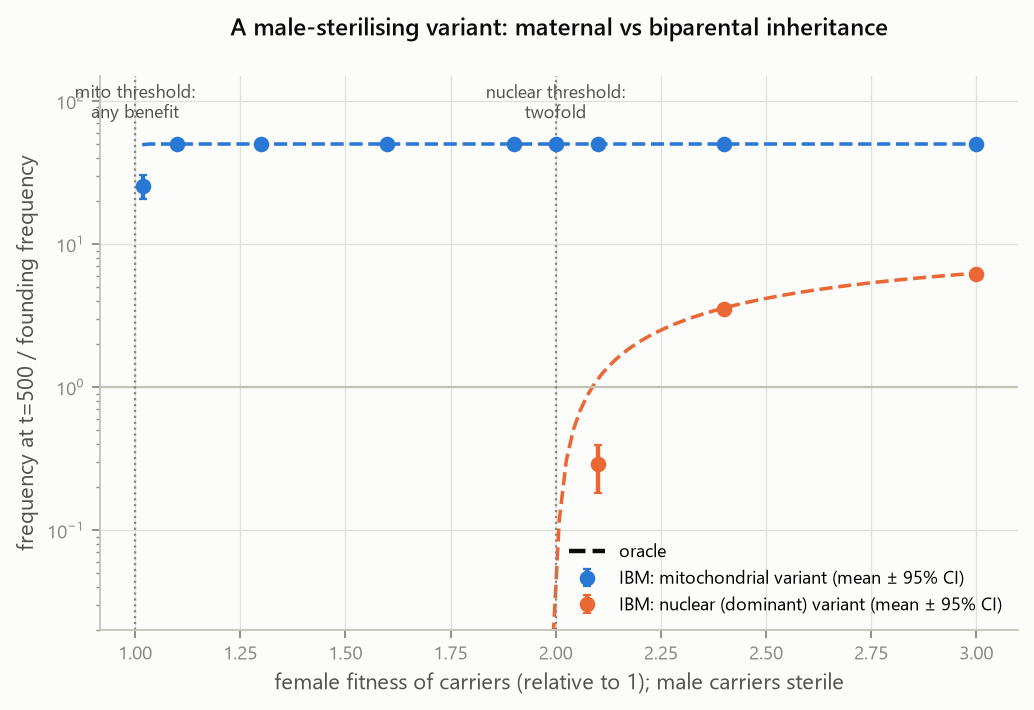
\includegraphics[width=0.49\textwidth]{C2_twofold_rule.png}\hfill
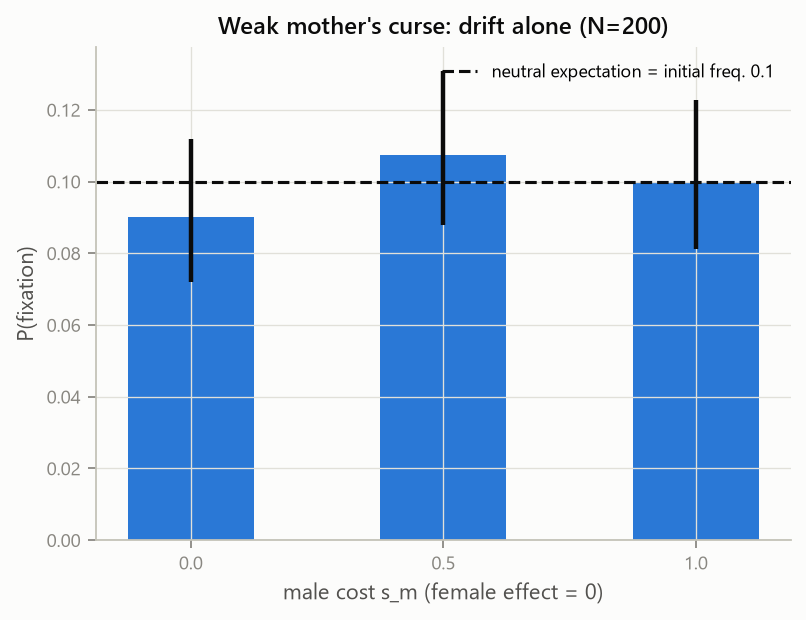
\includegraphics[width=0.49\textwidth]{C3_weak_mothers_curse.png}
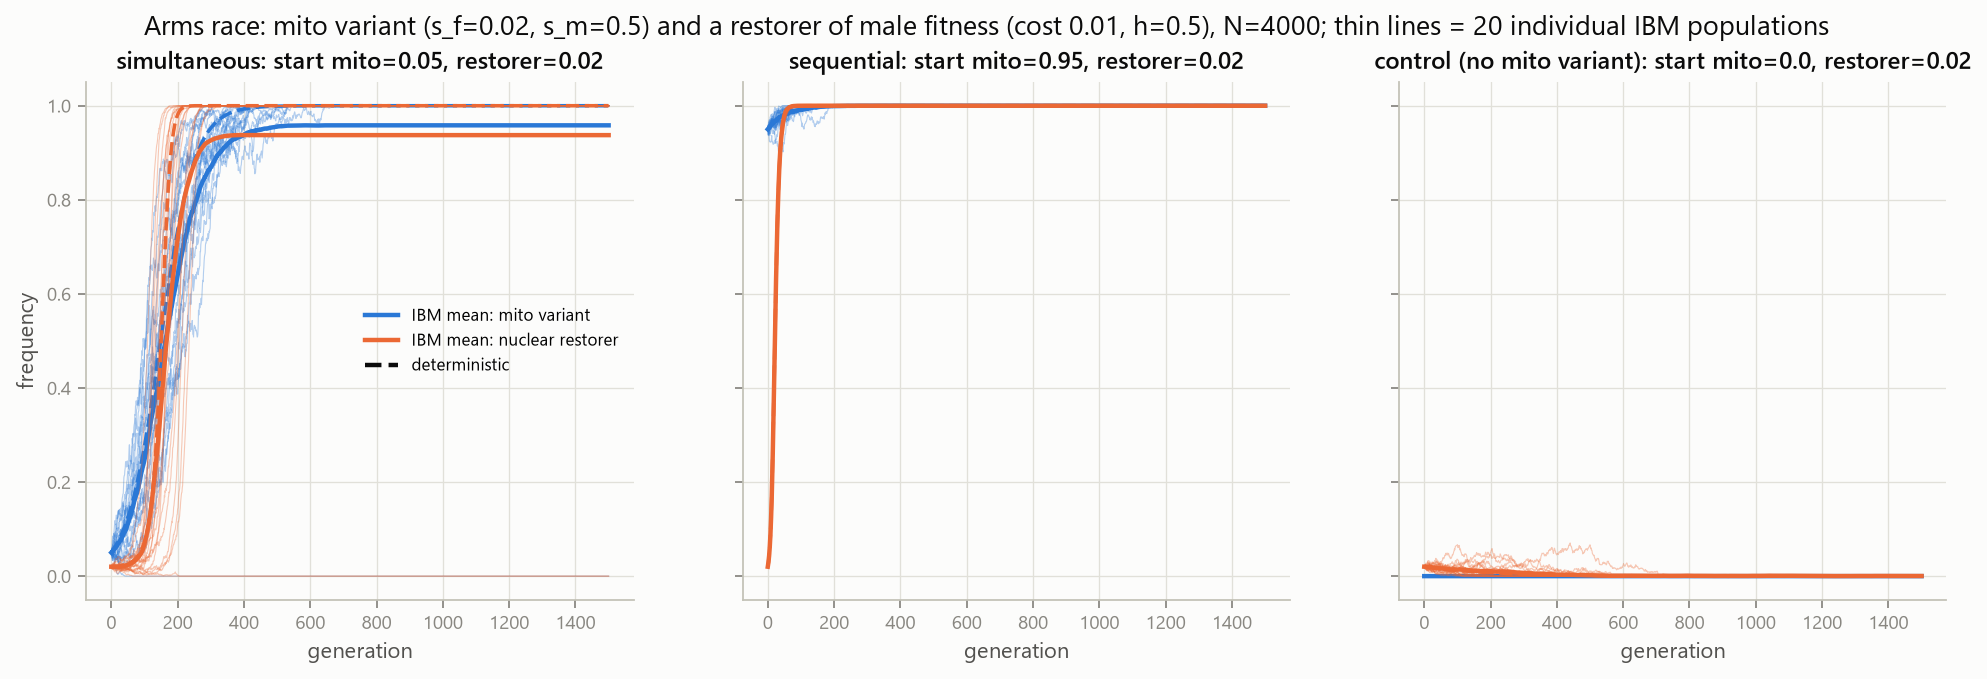
\includegraphics[width=\textwidth]{C4_restorer.png}
\caption{Twofold rule; weak form; restorer arms race (thin lines: individual \IBM\ populations).}\end{figure}

%=====================================================================
\section{Extended suite: classical SA theory, drift theory, ML}\label{sec:ext}
\subsection{Protected polymorphism (Kidwell 1977; Rice 1984; Fry 2010)}
Let $A_1$ be male-beneficial. Male fitnesses are $(1,\,1-h_ms_m,\,1-s_m)$ and female fitnesses $(1-s_f,\,1-h_fs_f,\,1)$ for $A_1A_1, A_1A_2, A_2A_2$. Applying Parsons' root at both boundaries gives, \emph{exactly}:
\begin{align}
\text{autosomal (Fry eq.\ 3): }&\ \frac{h_f}{1-h_m+h_fs_f}<\frac{s_m}{s_f}<\frac{1-h_f}{h_m(1-s_f)},\\
\text{X-linked (Rice eq.\ 2): }&\ \frac{2h_f}{1+h_fs_f}<\frac{s_m}{s_f}<\frac{2(1-h_f)}{1-h_fs_f}.
\end{align}
These identities were verified in 20{,}000 random parameter sets. The additive case reduces to Kidwell's wedge $1/(1+s_f)<s_m/s_f<1/(1-s_f)$.

\begin{table}[H]\centering\small\caption{Protected-polymorphism area in $(s_f,s_m)\in[0.02,0.3]^2$. \IBM\ verdicts come from two rare-invasion experiments per cell; M1 is the GP denoiser.}
\begin{tabular}{llccccc}\toprule
genome & dominance & oracle area & GP-\IBM\ area & IoU (GP) & IoU (raw) & cells agreeing\\\midrule
autosomal & additive & 0.187 & 0.170 & 0.896 & 0.681 & 100\% (134/144)\\
X & additive & 0.103 & 0.084 & 0.794 & 0.430 & 100\% (60/64)\\
autosomal & reversal $h=0.25$ & 0.770 & 0.736 & 0.955 & 0.888 & 100\% (130/144)\\
X & reversal $h=0.25$ & 0.494 & 0.457 & 0.913 & 0.722 & 98.2\% (56/64)\\
autosomal & $h_f=0.2,h_m=0.8$ & 0.187 & 0.177 & 0.893 & 0.520 & 100\% (126/144)\\
X & $h_f=0.2$ & 0.565 & 0.523 & 0.924 & 0.811 & 98.3\% (58/64)\\\bottomrule
\end{tabular}\end{table}

The \IBM\ reproduces the Rice--Fry debate:
\begin{itemize}
\item under Rice's assumption $h_m=1-h_f$ the autosomal area is independent of dominance;
\item the X is favoured only when the male benefit is recessive;
\item autosomes win for additive effects and for beneficial dominance reversal.
\end{itemize}
Emergent \IBM\ regions are 5--18\% smaller than the deterministic ones, in line with the finite-population argument of Mullon \emph{et al.}

\begin{figure}[H]\centering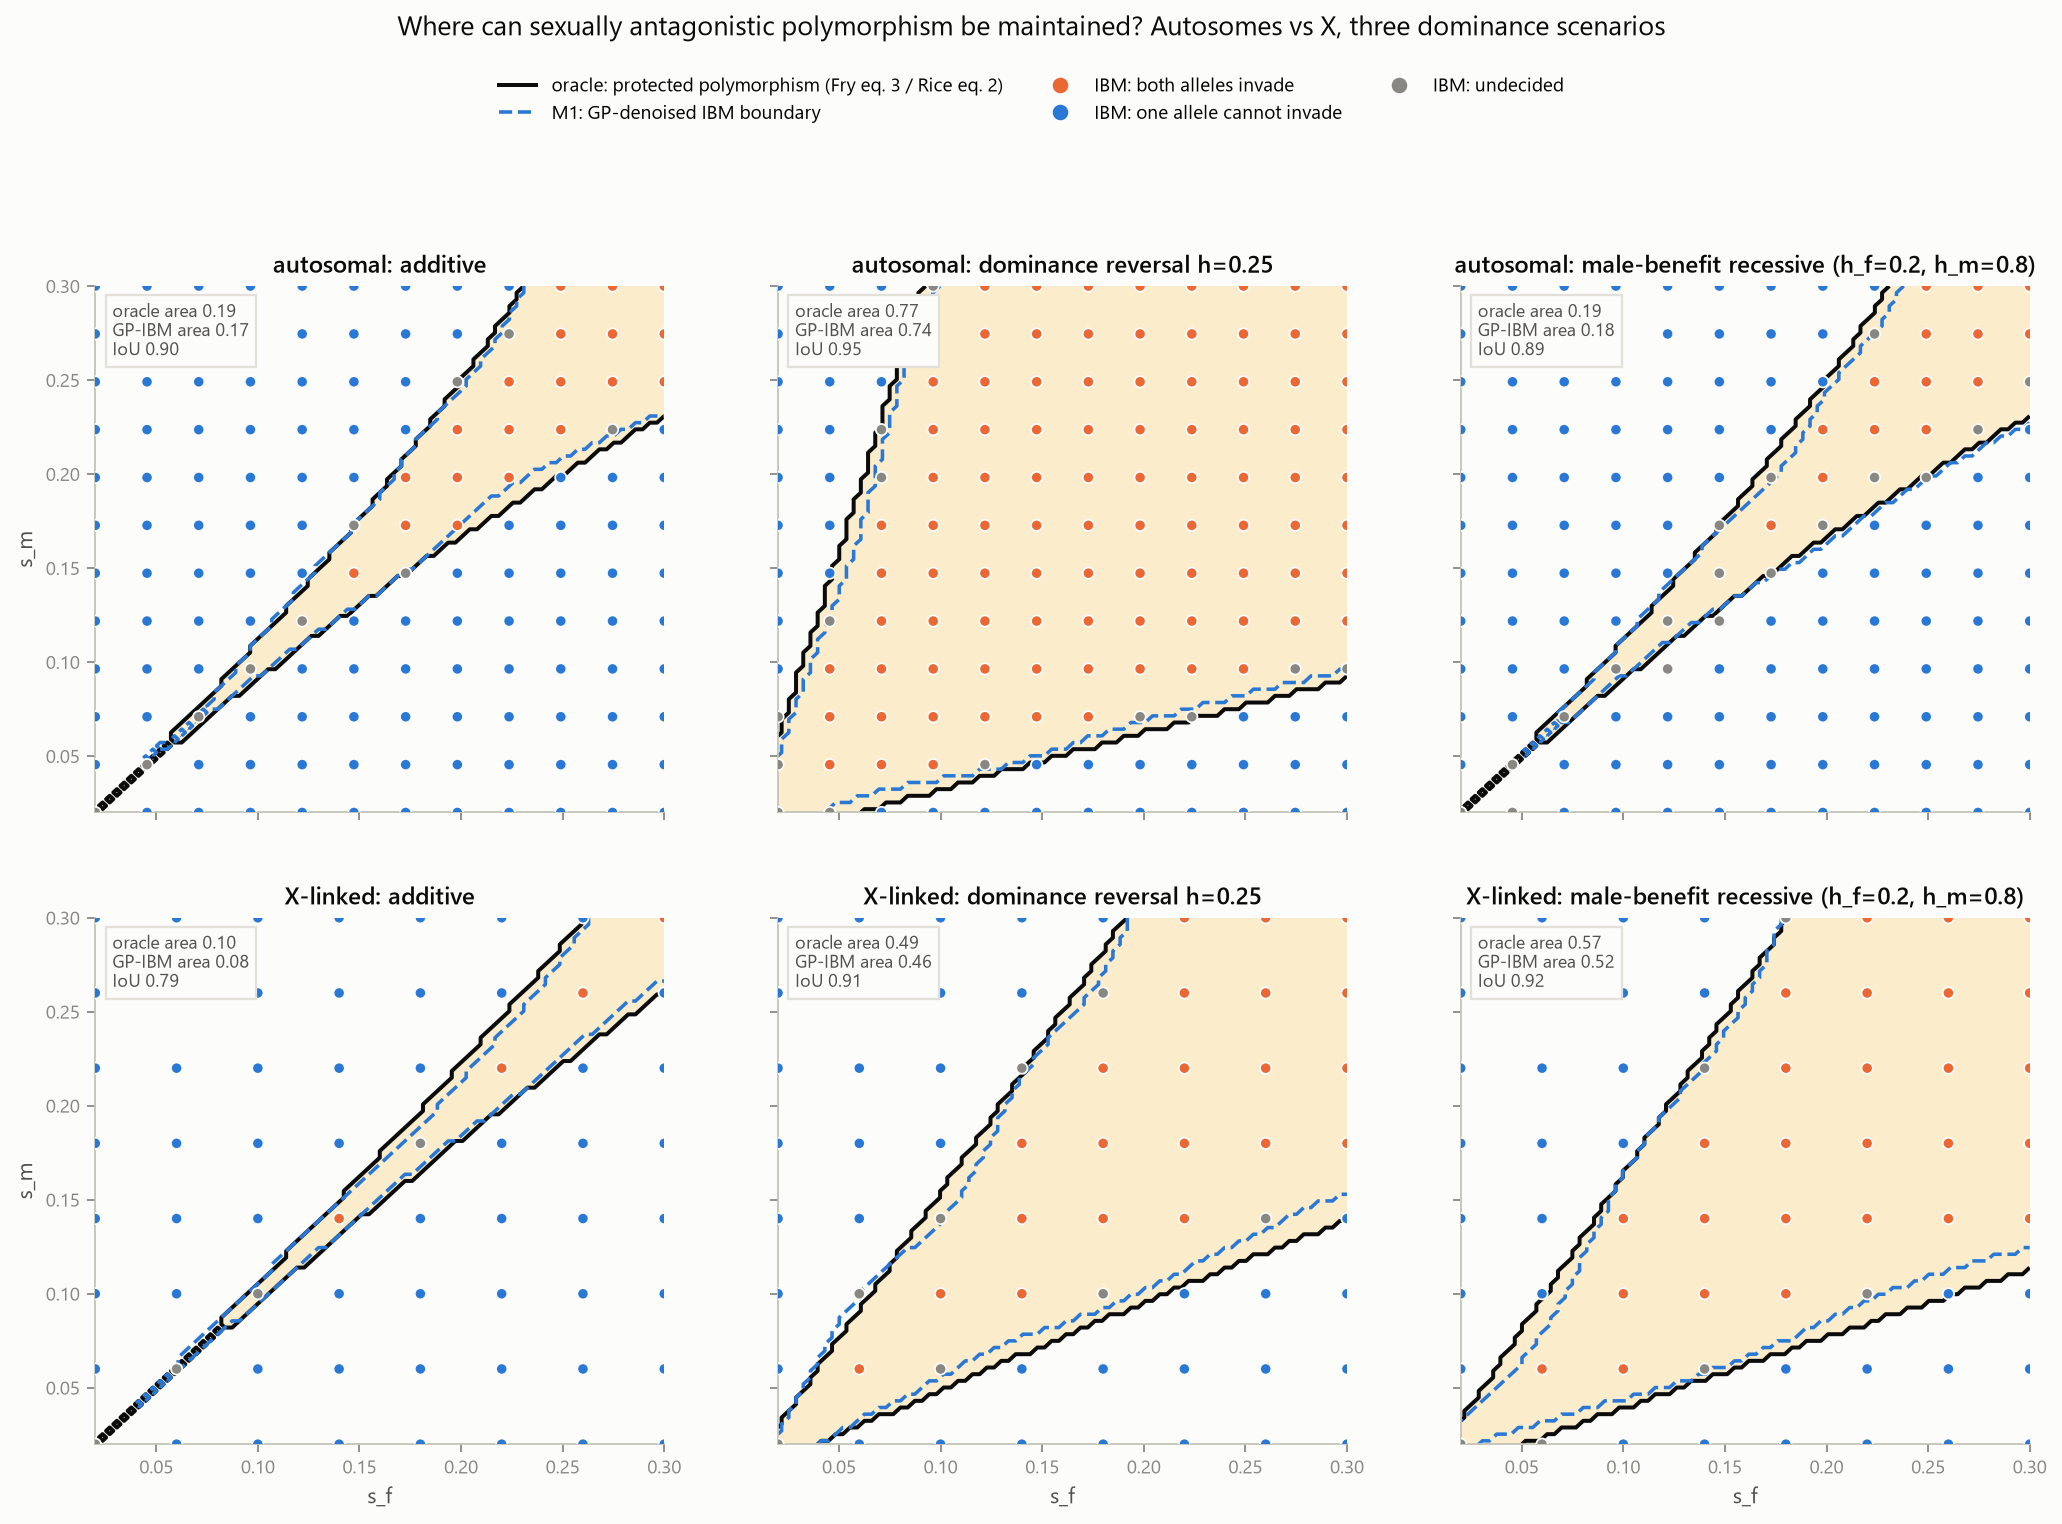
\includegraphics[width=\textwidth]{E1_E2_polymorphism_maps.png}
\caption{Oracle region (shaded, black boundary), GP-denoised \IBM\ boundary (dashed) and per-cell \IBM\ verdicts.}\end{figure}

\subsection{Fixation probabilities: Kimura and its correction}
Kimura's formula is $u(p)=(1-e^{-4Nsp})/(1-e^{-4Ns})$ with $s=\bar s=(s_f+s_m)/2$. For the mito variant the haploid form applies, with $N_e=N/2$. The general diffusion fixation probability is
\begin{equation}
u(p_0)=\frac{\int_0^{p_0}\psi}{\int_0^1\psi},\qquad \psi(y)=\exp\Big(-\!\int_0^y\frac{2M}{V}\Big),
\end{equation}
where $M(p)$ comes from the complete sex-specific recursion and $V=pq/2N$. This formula recovers Kimura's to $10^{-7}$ in the weak-selection limit.

Expanding the recursion gives $\Delta p\approx pq[\bar s-p(s_f^2+s_m^2)]$. The second-order term vanishes for a rare allele but opposes fixation as the allele becomes common; it is the term that creates Kidwell's wedge.
\begin{table}[H]\centering\small\caption{IBM fixation probabilities ($p_0=0.05$, $N=200,500,800$; 800 populations per point).}
\begin{tabular}{lcccc}\toprule
selection & RMSE vs Kimura & within 2 SE & RMSE vs full diffusion & within 2 SE\\\midrule
concordant & 0.010 & 100\% & 0.010 & 100\%\\
maternal mito ($N_e=N/2$) & 0.005 & 100\% & 0.005 & 100\%\\
antagonistic ($s_f-s_m=0.1$) & 0.083 & 0\% & 0.013 & 86\%\\\bottomrule\end{tabular}\end{table}
\begin{figure}[H]\centering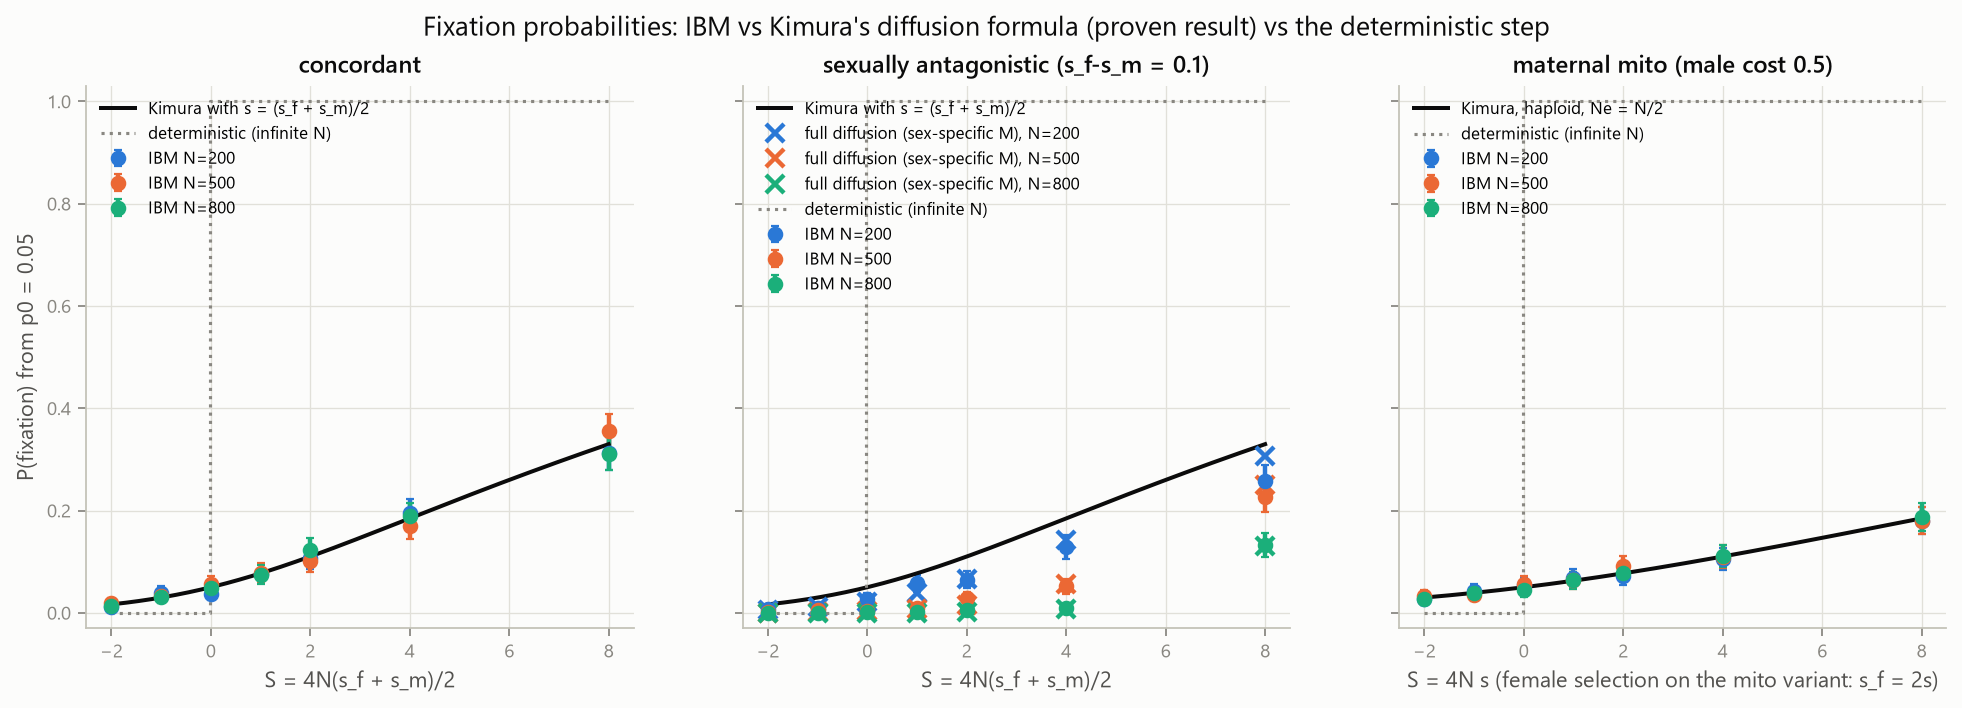
\includegraphics[width=\textwidth]{E3_kimura.png}\caption{IBM vs Kimura vs full diffusion vs the deterministic step.}\end{figure}

\subsection{Linkage to the sex-determining region (Rice 1987)}
The new recursion tracks $A_1$ on X in eggs, on X-sperm and on Y-sperm, with crossover $r$ between the SA locus and the SDR. At $r=1/2$ it reduces exactly to the autosomal model, which is tested. The new \IBM\ kernel determines sex genetically: an individual is male if it inherited its father's Y.
\begin{itemize}
\item Agreement with the oracle on whether polymorphism is maintained: \textbf{95.8\%}.
\item The polymorphic fraction falls from 0.75 at $r=0$ to 0.13 at $r=0.5$ (oracle); the \IBM\ gives 0.75 and 0.16.
\item The RMSE of the Y$-$X frequency difference is 0.021.
\end{itemize}
\begin{figure}[H]\centering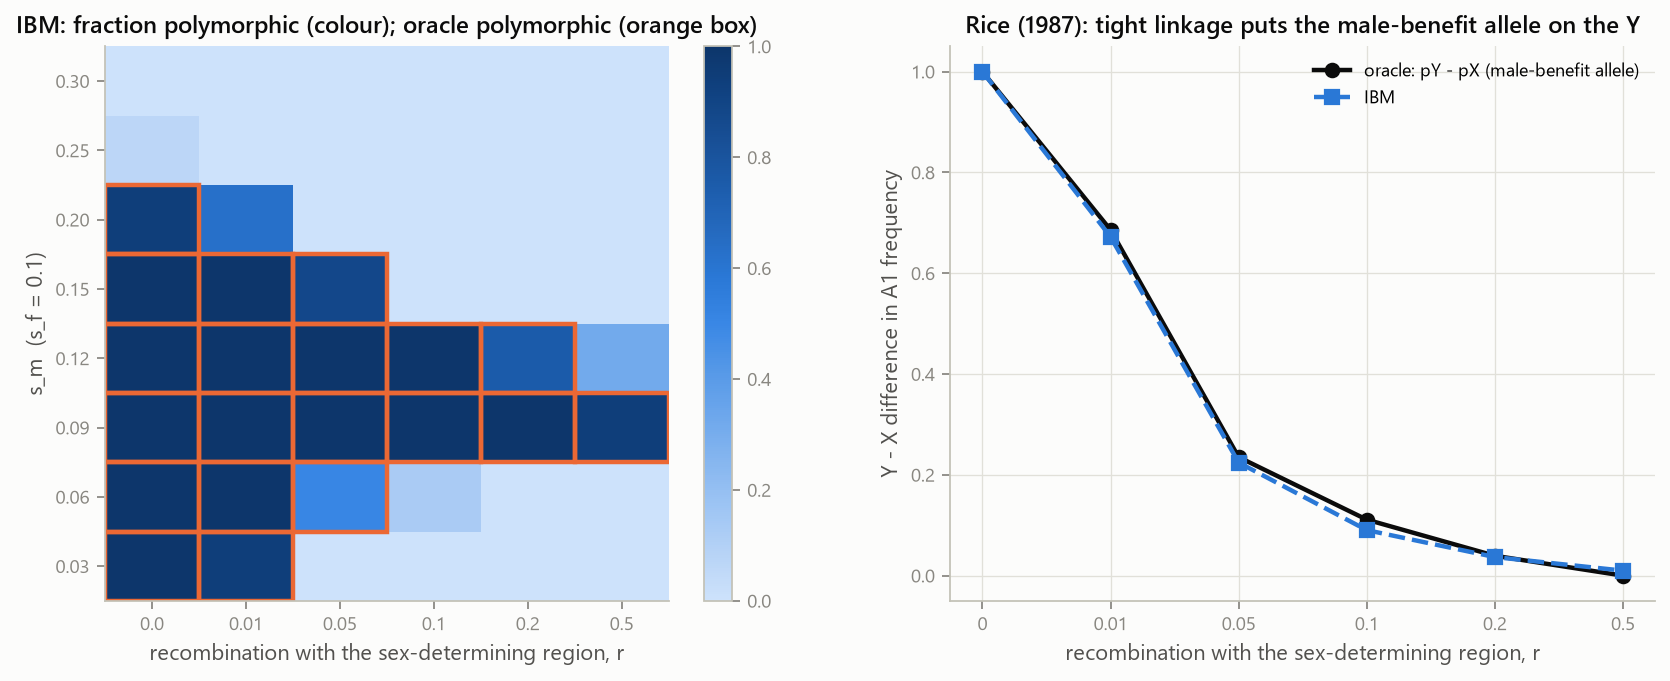
\includegraphics[width=0.95\textwidth]{E4_xy_linkage.png}\caption{XY linkage: polymorphism region vs $r$, and Y--X differentiation.}\end{figure}

\subsection{Diffusion time to loss of IaSC}
The backward Kolmogorov equation $\tfrac12V T''+MT'=-1$ was solved by finite differences on 4{,}001 nodes ($M$ from the poster's one-locus map, $V=pq/N_e$).
\begin{itemize}
\item With $N_e=N$: median relative error 11.5\% (max 27\%).
\item \textbf{Tuner:} measuring $N_e$ from the \IBM's own one-step fluctuations gives $N_e/N=0.896$ (random survival adds variance). This cuts the error to a median of \textbf{3.7\%} (max 8.5\%).
\item Mean persistence grows roughly exponentially with $N$ in the middle of the $a$-range: 497 generations at $N=200$ against 38{,}000 at $N=800$ for $a=0.2$.
\end{itemize}
\begin{figure}[H]\centering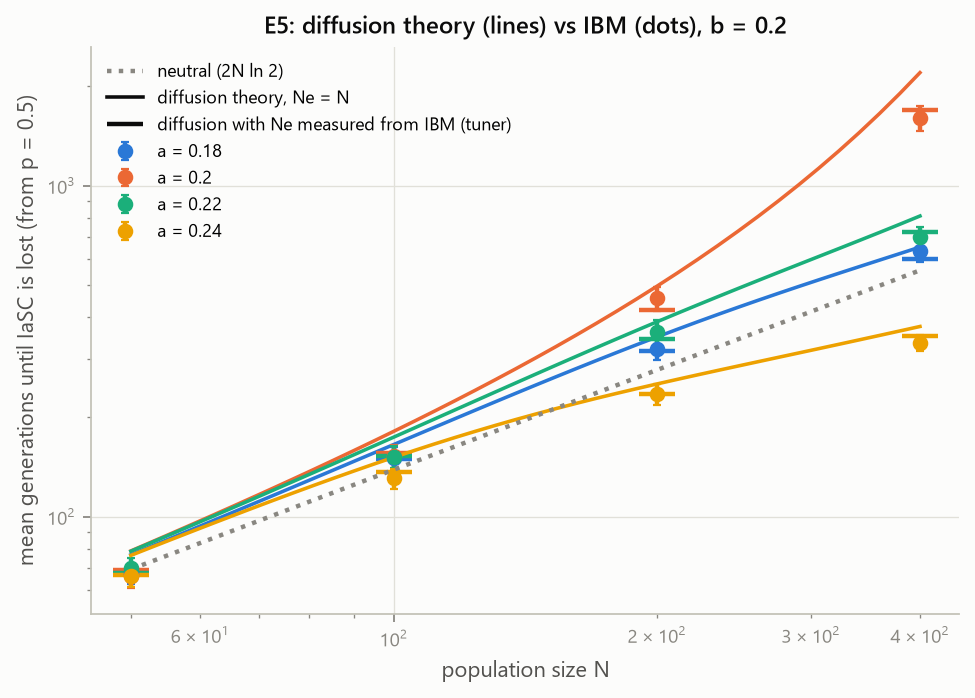
\includegraphics[width=0.62\textwidth]{E5_diffusion_persistence.png}\caption{Diffusion theory (lines), calibrated diffusion (dashes) and \IBM\ (dots).}\end{figure}

\subsection{ML layer (analysis only)}
\begin{description}
\item[M1, GP denoiser.] Heteroscedastic GP regression on $\tanh(\tfrac12\log\text{ratio})$, with a variance floor and a length-scale lower bound equal to the grid spacing. Without these constraints, cells with zero reported variance collapsed the length scale and inflated the region (IoU 0.004 in a first attempt). After the fix, IoU is 0.79--0.96, above the raw-grid IoU in all six cases.
\item[M2, neural emulator.] An MLP was trained on \IBM\ fixation data for $N\le600$ and tested at $N=800$.
  \begin{itemize}
  \item With inputs $(\log N,s)$ the RMSE vs Kimura is 0.046.
  \item With the diffusion scaling input $Ns$ it is \textbf{0.010}, closer to Kimura than the raw \IBM\ estimates (0.021).
  \end{itemize}
  The data therefore exhibit Kimura's $Ns$ collapse, and the emulator acts as a denoiser.
\item[M3, inverse problem.] We recovered $(s_f,s_m)$ from one 100-generation trajectory.
  \begin{itemize}
  \item At $N=5000$: amortised MLP RMSE 0.012/0.014, against 0.030/0.031 for the oracle least-squares fit.
  \item At $N=500$: 0.037/0.034 against 0.099/0.100. The oracle fit hits its bounds because drift is unmodelled.
  \item The difference $s_f-s_m$ is better identified than either coefficient (oracle 0.0098 at $N=5000$).
  \end{itemize}
\end{description}
\begin{figure}[H]\centering
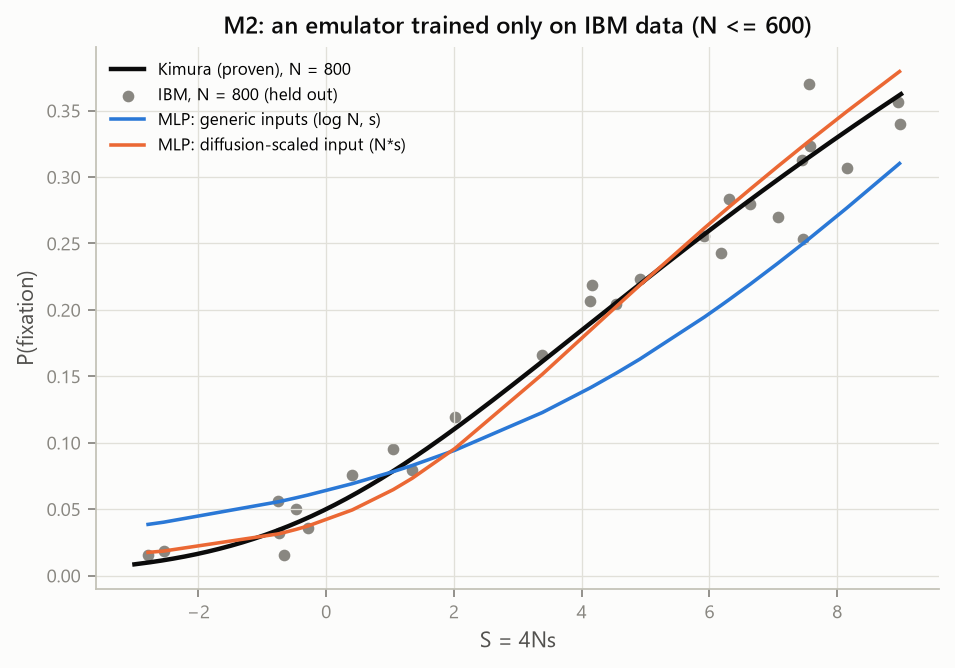
\includegraphics[width=0.44\textwidth]{M2_emulator.png}\hfill
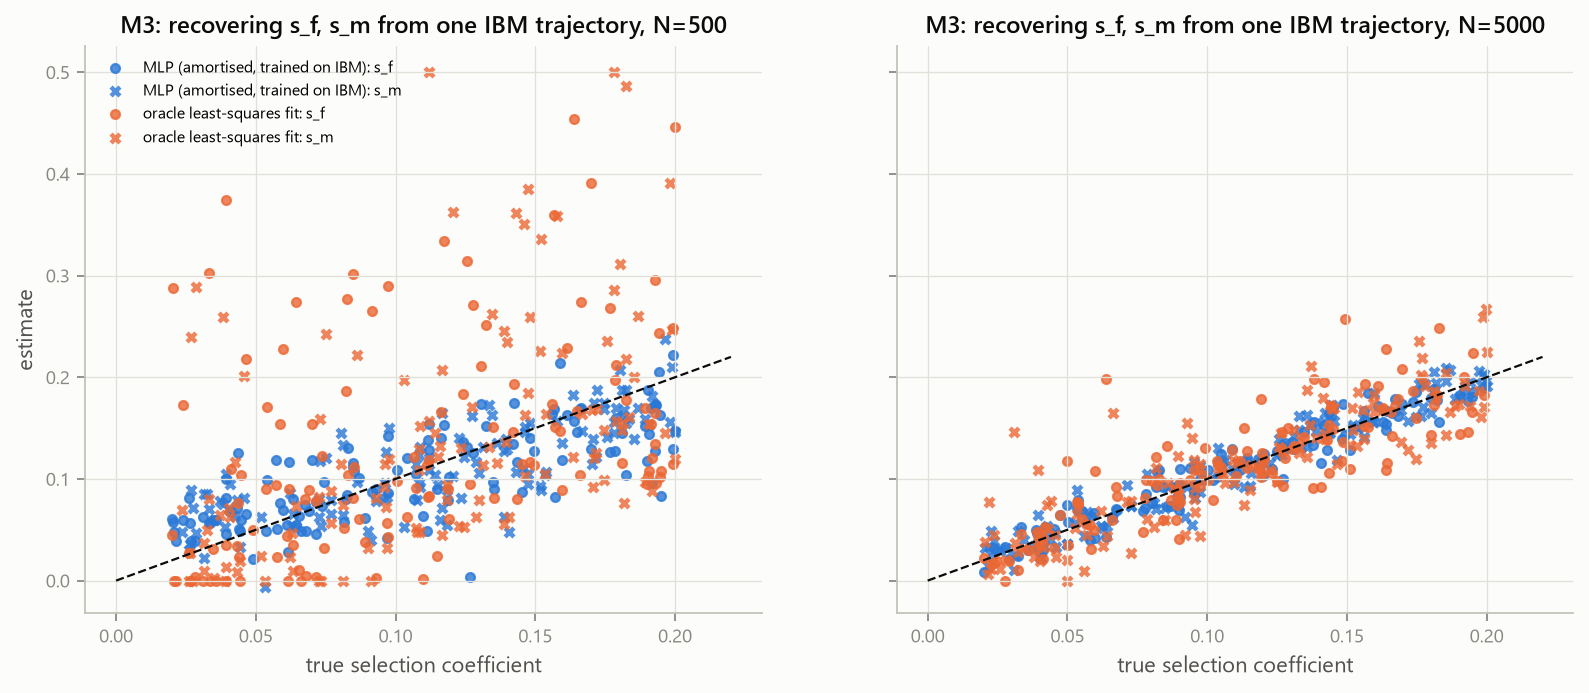
\includegraphics[width=0.55\textwidth]{M3_inverse_problem.png}
\caption{M2 emulator vs Kimura (held-out $N$); M3 parameter recovery.}\end{figure}

%=====================================================================
\section{Computation and reproducibility}
\begin{itemize}
\item Python 3.14, numpy 2.5, scipy 1.18, numba 0.68, sympy 1.14, pandas/pyarrow, scikit-learn 1.9 and matplotlib 3.11.
\item The optional OpenCL backend runs on the Radeon RX 560X. ROCm/HIP, CUDA and JAX are unavailable for Polaris on Windows.
\item Throughput: CPU $\approx3.8\times10^{7}$ and GPU $2.7$--$3.8\times10^{8}$ individual-generations/s.
\item Runs default to $N_\text{cpu}-2$ threads at below-normal priority.
\item There are 36 automated tests: zero leakage, formula identities, symbolic vs finite-difference Jacobians, compiled vs reference iterators, \IBM\ neutrality, recombination and maternal transmission, GPU/CPU statistical equivalence, and the GP denoiser on synthetic data.
\item Seeds, parameters, tables (Parquet) and figures are written under \texttt{results/}; \texttt{scripts/run\_all.py} reproduces everything.
\end{itemize}

\section{Conclusions}
\begin{enumerate}
\item Wherever their assumptions hold, the deterministic results of every source (poster, Parsons, Owen, Kidwell/Rice/Fry, Rice 1987) emerge from populations of individuals that never see the equations.
\item The departures are systematic and predicted by stochastic theory: drift erodes weak balancing selection; thresholds become probabilities; and Kimura's sex-averaging fails under strong antagonism, while the full diffusion corrects it.
\item For the poster: resolution of IaSC by modifiers is robust qualitatively. Quantitatively, it depends on whether the conflict survives long enough, which is set by $N$ and by the restoring eigenvalue $\mu$, extremely close to 1 near the edges of the $a$-range.
\end{enumerate}

\section*{References}
\small
Fry JD (2010) The genomic location of sexually antagonistic variation: some cautionary comments. \emph{Evolution} 64:1510--1516.\\
Havird JC \emph{et al.}\ (2019) Selfish mitonuclear conflict. \emph{Curr Biol} 29:R496--R511.\\
Kidwell JF \emph{et al.}\ (1977) Regions of stable equilibria for models of differential selection in the two sexes under random mating. \emph{Genetics} 85:171--183.\\
Kimura M (1962) On the probability of fixation of mutant genes in a population. \emph{Genetics} 47:713--719.\\
Morrow EH, Arnqvist G, Pitnick S (2003) Adaptation versus pleiotropy: why do males harm their mates? \emph{Behav Ecol} 14:802--806.\\
Mullon C, Pomiankowski A, Reuter M (2012) The effects of selection and genetic drift on the genomic distribution of sexually antagonistic alleles. \emph{Evolution} 66:3743--3753.\\
Owen ARG (1953) A genetical system admitting of two distinct stable equilibria under natural selection. \emph{Heredity} 7:97--102.\\
Parsons PA (1961) The initial progress of new genes with viability differences between sexes and with sex linkage. \emph{Heredity} 16:103--107.\\
Rice WR (1984) Sex chromosomes and the evolution of sexual dimorphism. \emph{Evolution} 38:735--742.\\
Rice WR (1987) The accumulation of sexually antagonistic genes as a selective agent promoting the evolution of reduced recombination between primitive sex chromosomes. \emph{Evolution} 41:911--914.\\
Samant M, Moitra P, Sinha S, Prasad NG. A two-locus haploid model for the resolution of intra-locus sexual conflict (poster, IISER Mohali).
\end{document}
